\chapter{Einführung}

  \section{Motivation}
  \begin{itemize}
   \item effiziente Algorithmen vs. ineffiziente Algorithmen (also: polynomiell vs. super-polynomiell)
   \item Warum beschäftigen wir uns mit ineffizienten Algorithmen? Damit wir NP-schwere Probleme angehen können.
   \item Um mit NP-schweren Problemen umgehen zu können, bedient man sich:
   \begin{itemize}
    \item Näherungsverfahren
    \begin{itemize}
     \item Approximationsalgorithmen
     \item Heuristiken
    \end{itemize}
    \item Exakte Verfahren
    \begin{itemize}
     \item exakte exponentielle Algorithmen
     \item parametrisierte Algorithmen, also Laufzeiten der Form $f(k)\cdot poly(n)$
    \end{itemize}
   \end{itemize}
   \item Warum haben wir Interesse an exakten Verfahren?
   \begin{itemize}
    \item (Laufzeit nicht entscheidend)
    \item nicht-approximierbare Probleme
    \item moderate Eingabegröße
    \begin{itemize}
     \item z.B.: $n^3 > 1,0941^n \cdot n$ für $n \leq 100$
     \item TSP exakt lösbar für $n\leq 2000$ (für euklidsche Instanzen sogar bis 15000)
     \item $2^{100}\cdot n > 2^n$ für $n \leq 100$
    \end{itemize}
    \item Entscheidungsprobleme (z.B.: Hamiltonkreis)
    \item theoretisches Interesse
   \end{itemize}
   \item Thema: geht es intelligenter und schneller als Brute-Force?
   \item typisches Resultat: \\
   \begin{tabular}{lcr}
      BF: &$O(2^n)$ & $O^*(2^n)$\\ 
      Alg1: &$O(n\cdot 1,5^n)$ &$O^*(1,5^n)$\\ 
      Alg2: &$O(n^2\cdot 1,4^n)$ &$O^*(1,4^n)$\\
   \end{tabular}
   \item Wozu solche Ergebnisse?
   \begin{align*}
    a^{n_0'} &= c\cdot a^{n_0}\\
    n_0' \cdot \log a &= \log c + n_0 \log a\\
    n_0' &= \frac{\log c}{\log a} + n_0\\
   \end{align*}
   $\Rightarrow$ mehr Rechenleistung bringt nicht immer die gewünschte Laufzeitverbesserung, aber:
   \begin{align*}
    a^n, b^n, &a < b\\
    a^{n_0'} &= b^{n_0}\\
    n_0' &= \frac{\log b}{\log a} n_0\\
   \end{align*}
   \item Literatur: \textit{Exact Exponential Algorithms} von Fomin/Kratsch.
  \end{itemize}
  
  \begin{definition}[$O^*$-Notation]
   \[f(n) = O^*(g(n)) \Leftrightarrow f(n) = O(g(n)\cdot poly(n))\]
   Mathematische Definition aus der Übung:
   \[f(n) \in O^*(g)) \Leftrightarrow  \exists c,d,n_o \in \mathbb{N}: \forall n \geq n_0: 0 \leq f(n) \leq c\cdot n^d\cdot g(n)\]
   z.B: $O(1,498^n\cdot n^{100}) \subsetneq O(1,499^n)$
  \end{definition}

\begin{section}{Der Held-Karp-Algorithmus für TSP}

  Gegeben seien \(n\) Städte \(c_1, ..., c_n\) und für jedes Paar \(c_i \neq c_j\) eine Distanz \(d(c_i,c_j)\). Wir suchen eine Permutation (Rundtour) \(\Pi\) auf \(\{1,...,n\}\), sodass die Gesamtlänge der Tour 
  \[\left( \sum_{i=1}^{n-1} d(c_{\Pi(i)},c_{\Pi(i+1)}) \right) + d(c_{\Pi(n)},c_{\Pi(1)})\] 
  minimal ist.

  Ein brute-force-Algorithmus würde alle Permutation ausprobieren und damit Laufzeit \(O(n! \cdot n)\) haben. Dies ist eine exponentielle Laufzeit, denn es gilt
  \begin{align*}
    \Theta(n!\cdot n) &= n\cdot 2^{\Theta(n \cdot \log_2 n)}\\
    2^{O(n \log n)} = (\frac{n}{2})^{\frac{n}{2}} &\leq n! \leq n^n = 2^{n\log n}
  \end{align*}
  
  \underline{Dynamisches Programm}\\
  Für den Algorithmus von Held-Karp definieren wir \(\OPT[S,c_i]\) mit der nichtleeren Menge \(S \subseteq \{ c_2, ..., c_n \}\) und \(c_i \in S\) als Länge des kürzestens Weges von \(c_1\) nach \(c_i\), der genau die Städte \(S \cup \{ c_1 \}\) besucht. Damit ist für $|S| = 1$ gerade \(\OPT[\{c_i\},c_i] = d(c_1,c_i)\) und für $|S| \geq 2$:
  \[\OPT[S,c_i] = \min_{c_j \in S \setminus \{c_i\}} \{ \OPT[S \setminus \{ c_i \}, c_j ] + d(c_j,c_i)\}.\]

  \begin{algorithm}[H]
    \caption{Algorithmus von Held-Karp zum Lösen von TSP}

    \KwName{Algorithmus von Held-Karp} \\
    \KwData{Städte \(c_1,...,c_n\) und Distanzfunktion \(d\)}
    \KwResult{Länge der kürzesten Rundreise durch alle \(c_i\)}

    \For{\(i = 1\) bis \(n\)}{
      \(\OPT[\{c_i\},c_i] \leftarrow d(c_1,c_i) \)
    }

    \For{\(j = 2\) bis \(n\)}{
      \For{\(S \subseteq \{ c_2,....,c_n \}\) mit \(|S| = j\)}{
        \For{\(c_i \in S\)}{
          \(\OPT[S,c_i] \leftarrow \min_{c_j \in S \setminus \{c_i\}} \{ \OPT[S \setminus \{ c_i \}, c_j ] + d(c_j,c_i)\}\)
        }
      }
    }

    \Return \(\displaystyle \min_{i \in \{2,...,n\}} \{ \OPT[\{c_2,...,c_n\},c_i] + d(c_i,c_1) \}\)
  \end{algorithm}

  \underline{Laufzeit} von Held-Karp:\\
  Der innere Ausdruck der For-Schleifen dauert $O(n)$. Dieser wird für höchstens alle Paare $(S,c_i)$ mit $S \subseteq \{c_2, \dots, c_n\}$ und $c_i \in S$ ausgewertet. Davon gibt es $O(n \cdot 2^n)$ viele, da es $2^n$ Teilmengen gibt und jede dieser Teilmengen $O(n)$ viele Elemente hat. Damit ergibt sich eine Gesamtlaufzeit von $O(2^n \cdot n^2) \subseteq O^*(2^n)$.
  
  \underline{Speicherplatz}: $O(n\cdot 2^n)$
\end{section}

\begin{section}{Ein Branching-Algorithmus für Größte unabhängige Teilmenge (Maximum independent Set, MIS)}

  Es sei ein Graph \(G = (V,E)\) gegeben. Gesucht ist ein \(I \subseteq V\) maximaler Kardinalität, so dass keine zwei Knoten aus \(U\) adjazent in \(G\) sind.

  Ein brute-force-Algorithmus würde in \(O^*(2^n)\) alle möglichen Teilmengen ausprobieren. Stattdessen wollen wir einen Algorithmus für MIS angeben, der in \(O^*(3^{n/3}) = O^*(1.4423^n)\) liegt. Wir beobachten zunächst: Ist \(I\) eine maximale unabhängige Menge, so gilt:

  \begin{enumerate}[(i)]
   \item \(v \in I \implies N(v) \cap I = \emptyset\),
   \item \(v \notin I \implies |N(v) \cap I| \geq 1\),
   \item $N[v] \isDefinedBy N(v) + v: N[v]$ enthält immer einen Konten $y$ aus $I$ und kein anderer Knoten aus $N[y]$ liegt in $I$.
  \end{enumerate}

  \begin{algorithm}[H]
    \caption{Algorithmus zur Berechnung der Mächtigkeit einer größten unabhängigen Menge}

    \KwName{MIS} \\
    \KwData{Graph \(G = (V,E)\)}
    \KwResult{Mächtigkeit einer größten unabhängigen Menge}

    \uIf{\(|V| = 0\)}{
      \Return 0
    }\Else{
      wähle $v \in V$ mit geringstem Grad\\
      \Return 1 + \(\displaystyle \max_{y \in N[v]} \{ \text{\textit{MIS}}(G \setminus N[y]) \}\)
    }
  \end{algorithm}
  
  \underline{Analyse:}\\
  Die Ausführung korrespondiert zu einem Suchbaum. Die Laufzeit entspricht $O^*(\sharp\text{Knoten im Suchbaum})$. Knoten vom Grad $2$ können für die Laufzeit-Analyse ignoriert werden, da ein Pfad aus Grad-$2$ Knoten im Suchbaum höchstens $n$ lang sein kann. Es reicht also, den reduzierten Suchbaum zu betrachten. In diesem sind aber mindestens die Hälfte aller Knoten Blätter.\\
  \underline{Alternativ:}\\
  Sei $l$ ein Blatt im Suchbaum, dann sein $L(l)$ die Länge des Pfades von der Wurzel zu $l$. Dann gilt für die Laufzeit des Algorithmus:
  \[ O^*(\sharp\text{Knoten}) \subseteq O^*(\sum_{l \text{ Blatt}} L(l)) \subseteq O^*(\sum_{l \text{ Blatt}} n) = O^*(\sharp\text{Knoten})\]
  
  Für die Anzahl der Knoten im Baum gilt folgende Rekursionsgleichung:
  \begin{align*}
  B(n) &\leq \sum_{y \in N[v]} B(n-(d(y)+1))\\
  &\leq \sum_{y \in N[v]} B(n-(d(v)+1))\\
  &= (d(v) + 1) \cdot B(n-\underbrace{(d(v) + 1)}_{=: s})\\
  &= s \cdot B (n-s)
  \end{align*}
  
  Auflösen der Rekursionsgleichung durch Beweis per Induktion:
  \begin{align*}
  B(0) &= 1\\
  \text{Behauptung: } B(n) &= 3^{\frac{n}{3}}\\
  \text{Induktion: (IA) } B(0) &= 1 \leq 3^{\frac{n}{3}}\\
  B(n) &\overset{\text{(IA)}}{\leq} s\cdot 3^{\frac{n-s}{3}} = 3^{\frac{n}{3}} \cdot \frac{s}{3^\frac{s}{3}} \leq 3^{\frac{n}{3}}
  \end{align*}

  Dieser Algorithmus hat also Laufzeit \(O^*(1.4423^n)\).
\end{section}
  
\begin{section}{Anwenungsgebiete für exakte Algorithmen}
  \begin{subsection}{NP-Entscheidungsprobleme}
  Gegeben ist die Eingabe $x \in \{0,1\}^*$. Gesucht ist die Lösung $y \in \{0,1\}^*$ mit $|y| \leq m(|x|)$ für ein Polynom $m$ und $R(x,y) = true$, wobei $R$ ein polynomialzeit-berechenbare Relation ist.
  
  Der brute-force Ansatz hat eine Laufzeit von $O^* (2^{m(|x|)})$.
  \end{subsection}

  \begin{subsection}{NP-Optimierungsprobleme}
  Gegeben ist eine Eingabe $x$, gesucht ist eine zulässige Lösung $y$ mit $R(x,y) = true$ und $|y| \leq m(|x|)$. Ziel ist es, einen minimalen (maximalen) Zielfunktionswert $obj(x,y) \in \mathbb{N}^+$. Hierbei sind $R,m, obj$ polynomialzeit-berechenbare Funktionen und $m$ zusätzlich polynomiell.
  \end{subsection}
  
  \begin{subsection}{Teilmengenprobleme}
   Eine zulässige Lösung ist eine Teilmenge einer gegebenen Grundmenge der Kardinalität $n$, z.B. MIS. Brute-force Ansätze haben hier eine Laufzeit von $O^*(2^n)$ -- alle möglichen Teilmengen testen.
  \end{subsection}
  
  \begin{subsection}{Permutationsprobleme}
   Eine zulässige Lösung ist eine Permutation einer gegeben Grundmenge mit Kardinalität $n$, z.B. TSP. Brute-force Ansätze dafür laufen in $O^*(n!) = O^*(2^{O(n\log n)})$
  \end{subsection}
  
  \begin{subsection}{Partitionierungsprobleme}
   Eine zulässige Lösung ist eine Partitionierung einer gegeben Grundmenge mit Kardinalität $n$, z.B. Graph-Färbbarkeit. Brute-force: $O^*(n^n) = O^*(2^{n\log n})$.
  \end{subsection}
\end{section}

\begin{section}{Weitere Branching-Algorithmen}
  \underline{Allgemeine Form (Branch \& Reduce):}\\
  Ein Branching-Algorithmus besteht aus Branching- und Reduktionsregeln. 
  \begin{itemize}
   \item Branch-Regel: Unterscheide verschiedene Möglichkeiten und löse für jedes ein entsprechendes Teilproblem; gewinne daraus die Lösung für das Gesamtproblem.
   \item Reduce-Regel: Reduziere die Problemgröße; stop
  \end{itemize}
  Die \textit{Korrektheit} von Branching-Algorithmen wird oft nicht bewiesen, da sie sich direkt aus dem vorliegenden Code ergibt. Die \textit{Laufzeit} von Branching-Algorithmen analysiert man auf Basis der Anzahl der Blätter des Suchbaum.

  \begin{definition}[Branching-Vektor]
    Betrachte die Anwendung einer Branching-Regel $b$ auf einer Eingabe der Größe $n$. Angenommen, $b$ zerlegt die Probleminstanz in \(r \geq 2\) verschiedene Teilinstanzen der Größe $n - t_1, ..., n - t_r$, so heißt $(t_1,...,t_r)$ \textit{Branching-Vektor} von $b$. 
  \end{definition}
  
  Für die Laufzeit ergibt sich daher folgende Rekurrenzgleichung für $T(n)$: 
  \begin{align*}
    T(n) &\leq \sum_{i=1}^r T(n-t_i)\\
    T(0) &= 1
  \end{align*}
  für die Anzahl der Blätter.
  
  \begin{theorem} \label{satzLaufzeit}
    Sei \(b\) eine Branching-Regel mit Branching-Vektor \( (t_1,...,t_r) \). Dann führt die ausschließliche Anwendung von \(b\) zur Laufzeit \(O^*(\alpha^n)\), wobei \(\alpha\) die eindeutige positive relle Lösung der Gleichung 
    \[ x^t - x^{t-t_1} - x^{t - t_2} - ... - x^{t - t_r} = 0 \] 
    mit \(t = \max t_i, i \in [1,r]\) ist.
  \end{theorem}
  \begin{proof}
    Wir nehmen an: $T(n) = x^n$. Dann ergibt sich daraus:
    \[ x^n \overset{!}{=} x^{n-t_1} + x^{n-t_2}+\dots+x^{n-t_r}\]
    Division mit $x^{n-t}$ ergibt
    \[ x^t = x^{t-t_1}+x^{x-t_2}+\dots+x^{t-t_r}\]
    Zu zeigen bleibt noch, dass immer eine eindeutige relle positive Lösung existiert. 
  \end{proof}
  Problematisch dabei ist, dass die Lösung oft irrational ist und dass üblicherweise auf 5 Stellen gerundet wird. In Normalfall wird die Lösung mit $\tau(t_1,\dots,t_r)$ bezeichnet. Dieses $\tau$ nennt man auch \textit{Branching-Faktor}.
  
  \begin{lemma}
   Sei $r \geq 2$ und $t_i > 0$ für $i = 1,\dots,r$, dann gilt
   \begin{enumerate}[i)]
    \item  $\tau(t_1,\dots,t_r) > 1$
    \item $\tau(t_1,\dots,t_r) = \tau(t_{\pi(1)},\dots,t_{\pi(r)})$ für alle Permutationen $\pi$. Permutation der Fallreihenfolge ändert nichts an der Laufzeit, da es zum gleichen Suchbaum führt.
    \item $\tau(t_1,\dots,t_r) < \tau(t'_1,\dots,t_r)$ für $t_1 > t'_1$. Man sagt dann auch, $\tau(t'_1,\dots,t_r)$ \underline{dominiert} $\tau(t_1,\dots,t_r)$.
   \end{enumerate}
  \end{lemma}
  
  \begin{lemma}[Balancing-Lemma]
   \begin{enumerate}[i)]
    \item $\tau(k,k) \leq \tau(i,j)$ mit $2\cdot k = i+j$
    \item $\tau(i,j) < \tau(i+\varepsilon,j-\varepsilon)$ für $0<i<j$ und $0<\varepsilon< \frac{j-i}{2}$.
   \end{enumerate}
  \end{lemma}
  
  \textbf{Addition von Branching-Vektoren:}\\
  Wir wissen, dass im rechten Baum $\tau(i,j) > \tau(k,l)$ gilt. Dann lässt sich der Baum wie folgt vereinfachen:
  \[\begin{tikzpicture}
    \draw (0,0)node[](x1){i+k} (2,0)node[](x2){i+l}
	  (0,0.5)node[circle, draw](a1){} (2,0.5)node[circle,draw](a2){}
	  (1,1.5)node[circle,draw](b1){} (3,1.5)node[circle,draw](b2){} (3,1)node[](x3){j}
	  (2,2.5)node[circle,draw](c1){};
    \path[fill,draw, postaction={decoration={text along path,text={k},text align ={left indent=10pt},raise=0.5ex},decorate}] (a1) -- (b1);
    \path[fill,draw, postaction={decoration={text along path,text={l},text align ={left indent=10pt},raise=0.5ex},decorate}] (b1) -- (a2);
    \path[fill,draw, postaction={decoration={text along path,text={i},text align ={left indent=10pt},raise=0.5ex},decorate}] (b1) -- (c1);
    \path[fill,draw, postaction={decoration={text along path,text={j},text align ={left indent=10pt},raise=0.5ex},decorate}] (c1) -- (b2);
  \end{tikzpicture}
   \overset{\wedge}{=}
   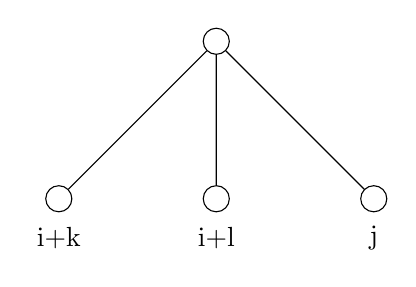
\begin{tikzpicture}
    \draw (0,0)node[]{i+k} (2,0)node[]{i+l} (4,0)node[]{j}
	  (0,0.5)node[circle, draw](a1){} (2,0.5)node[circle, draw](a2){} (4,0.5)node[circle, draw](a3){}
	  (2,2.5)node[circle, draw](b){};
    \filldraw (a1) -- (b) -- (a2);
    \filldraw (a3) -- (b);
   \end{tikzpicture}\]
   Mit der neuen Darstellung: $\tau(i+k,i+l,j)$.
  

\begin{subsection}{SAT}
  Eingabe ist eine aussagenlogische Formel in konjunktiver Normalform (KNF). Existiert eine erfüllende Belegung der Variablen? Ein brute-force-Algorithmus hat Laufzeit \(O^*(2^n)\); ob ein Algorithmus mit Laufzeit \(O^*( (2-\varepsilon)^n )\) existiert ist ungeklärt.
\end{subsection}
  
\begin{subsection}{$k$-SAT}
  Eingabe ist eine aussagenlogische Formel in konjunktiver Normalform, in der jede Klausel Länge kleiner oder gleich \(k\) besitzt. 
  
  Wir entwickeln für $k$-SAT einen Algorithmus mit Laufzeit $O^*(\alpha_k^n)$, wobei $\alpha_k < 2$.
  \begin{itemize}
   \item Der Algorithmus erweitert rekursiv partielle Belegungen der Variablen zu (ggf.) vollständingen Belegungen. 
   \item Falls $t$ eine partielle Belegung einer Formel $F$ in KNF ist, dann ist $F[t]$ die \textit{reduzierte} Formel, die entsteht, indem man Klauseln streicht, die positive Literale enthalten und negierte Literale löschen. 
   \item Also ist $F[t]$ erfüllbar, genau dann wenn $t$ sich zu einer erfüllbaren Belegung erweitern lässt. 
   \item Enthält $F[t]$ leere Klauseln, so ist $F[t]$ nicht erfüllbar. 
   \item Ist $F[t]$ leer, so ist $F[t]$ erfüllt.
  \end{itemize}
  
  \begin{algorithm}[H]
    \caption{Algorithmus zur Entscheidung einer \(k\)-CNF-Formel \(F\)}

    \KwName{\(k\)-SAT1} \\
    \KwData{Formel \(F\) in konjunktiver Normalform und maximaler Klausellänge \(k\)}
    \KwResult{Erfüllbarkeit von \(F\)}

    \uIf{\(F\) enthällt leere Klausel}{
      \Return false
    }\ElseIf{\(F\) ist die leere Formel}{
      \Return true
    }

    wähle Klausel \(l = (l_1 \vee l_2 \vee ... \vee l_q)\)\;
    $t_1 \leftarrow l_1 = true$\; 
    $t_2 \leftarrow l_1 = false, l_2 = true$\;
    \vdots
    $t_q \leftarrow l_1 = false, \dots, l_{q-1} = false, l_q = true$\; 
    \Return \(k\)-SAT1(\(F[t_1])\)) \(\vee\) \(k\)-SAT1(\(F[t_2])\)) \(\vee\) ... \(\vee\) \(k\)-SAT1(\(F[t_q])\))\;
  \end{algorithm}

  Für die Laufzeit ergibt sich die rekursive Formel \(T(n) \leq T(n-1) + T(n-2) + ... + T(n-q)\) mit einem \(q \leq k\). Die Laufzeit ergibt sich dann nach Satz \ref{satzLaufzeit} als $O^*(\beta_k^n)$, für \(3\)-SAT beispielsweise \(O^*(1.8393^n)\).

  \paragraph{Verbesserung.} Wir modifizieren den Algorithmus zu \(k\)-SAT2, indem wir immer die kleinste Klausel wählen. Dazu benötigen wir die folgende Definiton:
  \begin{definition}
  Wir nennen eine partielle Belegung \(t\) einer Formel \defNotion{autark}, wenn jede Klausel, die mindestens ein von \(t\) belegtes Literal enthält, auch ein von \(t\) mit wahr belegtes Literal enthält. Dies bedeutet, dass die Klausel unabhängig von allen anderen Literalen der Klausel wahr ist. 
  \end{definition}
  \paragraph{Beispiel.}
  \[(x_1\vee x_2\vee \overline{x}_3) \wedge (\overline{x}_1 \vee \overline{x}_2) \wedge(\overline{x}_2 \vee \overline{x}_3 \vee x_4)\wedge (x_3 \vee \overline{x}_4)\]
  Für $t = \{x_1 = true, x_2 = false\}$ ergibt sich $F[t] = \{(x_3 \vee \overline{x}_4)\}$.\\
  Für $t' = \{x_1 = true\}$ ergibt sich $F[t'] = \{(\overline{x}_2) \wedge (\overline{x}_2 \vee \overline{x}_3 \vee x_4) \wedge (x_3 \vee\overline{x}_4)\}$

  Daraus ergeben sich die folgenden Beobachtungen.
  
  \begin{enumerate}[(i)]
   \item Wenn \(t\) autark ist, dann ist \(F\) genau dann erfüllbar, wenn \(F[t]\) erfüllbar ist. Das bedeutet, dass wir für autarke \(t\) das Ergebnis von \(k\)-SAT2(\(F[t]\)) zurückgeben können.
   \item Wenn \(t\) nicht autark ist, dann enthält \(F[t]\) eine Klausel von Länge höchstens \(k-1\).
  \end{enumerate}
  
  Der verbesserte Algorithmus sieht dann wie folgt aus (Änderungen in {\color{red}rot}):
  
\end{subsection}
  \begin{algorithm}[H]
    \caption{Verbesserter Algorithmus zur Entscheidung einer \(k\)-CNF-Formel \(F\)}

    \KwName{\(k\)-SAT2} \\
    \KwData{Formel \(F\) in konjunktiver Normalform und maximaler Klausellänge \(k\)}
    \KwResult{Erfüllbarkeit von \(F\)}

    \uIf{\(F\) enthällt leere Klausel}{
      \Return false
    }\ElseIf{\(F\) ist die leere Formel}{
      \Return true
    }

    wähle {\color{red}kürzeste} Klausel \(l = (l_1 \vee l_2 \vee ... \vee l_q)\)\;
    $t_1 \leftarrow l_1 = true$\; 
    $t_2 \leftarrow l_1 = false, l_2 = true$\;
    \vdots
    $t_q \leftarrow l_1 = false, \dots, l_{q-1} = false, l_q = true$\; 
    {\color{red} 
      \uIf {$t_i$ autark für ein $i = 1,\dots,q$} {
	\Return $k$-SAT2($F[t_i]$)
      }
    }
    \Return \(k\)-SAT2(\(F[t_1])\)) \(\vee\) \(k\)-SAT2(\(F[t_2])\)) \(\vee\) ... \(\vee\) \(k\)-SAT2(\(F[t_q])\))\;
  \end{algorithm}
  \paragraph{Behauptung.} Der Algorithmus hat eine Laufzeit von $O^*(\alpha_k^n)$, wobei $\alpha_k = \beta_{k-1}$.
  \paragraph{Beobachtun.} Sei $v$ ein Knoten im Suchbaum, nicht die Wurzel. Wenn $v$ ein $k$-Branching ist, dann ist sein Vater ein Reduce-Knoten. (Immer, wenn gebranched wird, enthält Formel $F[t_i]$ mindestens eine Klausel der Länge $\leq k-1$.)
\end{section}
  
  